\section*{WRITING TASK 1}
You should spend about 20 minutes on this task.

\begin{quote}\large The chart shows the numbers of visitors to three museums in 2024. The table gives their average spending per visit in the same year.
\end{quote}
Describe the main features of the information, select relevant details, and make comparisons where appropriate.

\begin{center}
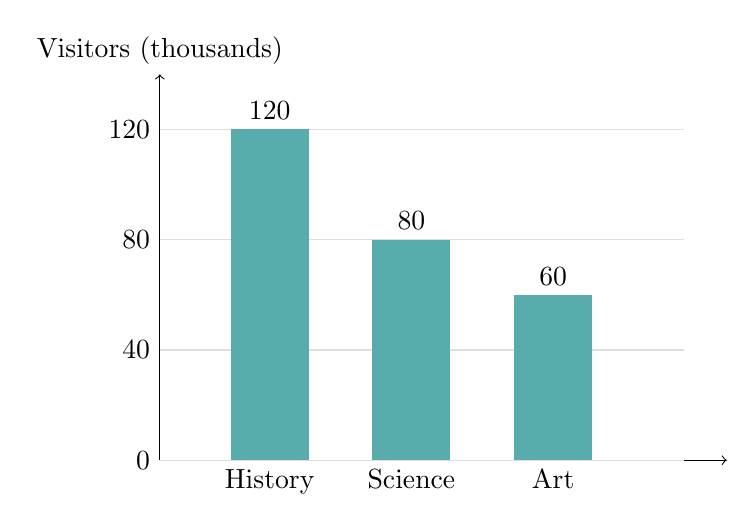
\begin{tikzpicture}[x=1.8cm,y=0.035cm]
\draw[->] (0,0)--(4,0);\draw[->] (0,0)--(0,140) node[above]{Visitors (thousands)};
\foreach \v in {0,40,80,120}{\node[left] at (0,\v){\v};\draw[gray!25] (0,\v)--(3.7,\v);}
\foreach \x/\v/\name in {0.5/120/History,1.5/80/Science,2.5/60/Art}{\fill[teal!65] (\x,0) rectangle +(0.55,\v);\node[above] at (\x+0.275,\v){\v};\node[below] at (\x+0.275,0){\name};}
\end{tikzpicture}
\par\bigskip\begin{tabular}{|l|r|}\hline Museum & Spending per visitor (USD)\\\hline History & 8\\Science & 15\\Art & 20\\\hline\end{tabular}
\end{center}
Write at least 150 words.
\par\bigskip
{\footnotesize\color{gray} Original practice material; fictional settings and data. Not an official IELTS examination paper.}
